
\begin{textarea}[]
	\only<1>{
		Not only does this force pulls you towards earth, it also pulls earth towards you, isn't that cool?
	}
	\only<2>{
		What is gravitation?
	}
\end{textarea}



\begin{textarea}[]
	\only<1>{
		This effect allows tennis, soccer and other ball sport player to add spin to their gaming device
	}
	\only<2>{
		What is the Magnus effect?
	}
\end{textarea}



\begin{textarea}[]
	\only<1>{
		\begin{columns}[c] 
			\column{.3\textwidth} 
			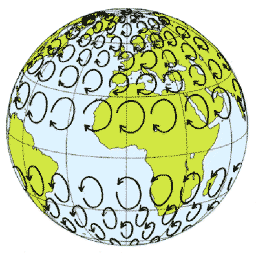
\includegraphics[height=1.0\linewidth]{categories/media/mayTheForce/Coriolis_effect14.png}
			\column{.5\textwidth}
			On the large scale, this force influences the atmospheric behavior, even snipers and other long-distance shooters have to take it into account.
		\end{columns}
	
	}
	\only<2>{
		What is the Coriolis effect?
	}
\end{textarea}

\begin{textarea}[]
	\only<1>{
		It's the force $\textbf{F}$ acting on a particle of electric charge $q$ with instantaneous velocity $\textbf{v}$, due to an external electric field $\textbf{E}$ and magnetic field $\textbf{B}$
		
		$\mathbf{F} = q(\mathbf{E} + \mathbf{v} \times \mathbf{B})$.
	}
	\only<2>{
		What is the Lorentz force?
	}
\end{textarea}

\begin{textarea}[]
	\only<1>{
		A law of physics that describes force interacting between static electrically charged particles.
			
		$F =k \frac{|q_1q_2|}{r^2}$.
	}
	\only<2>{
		What is the Coulomb Force?
	}
\end{textarea}  